Introduction \cite{huff_extensions_2014}.

\section{Micro Reactors}

\section{High Temperature Gas-cooled systems}

The high-temperature gas-cooled reactor concept benefits from the development of high-temperature reactors from 1970 to 1980 in the United States, France, Germany, and the United Kingdom. 
Among its advantages are:
- Achievement of higher temperatures (1000 C): This will improve electrical production efficiency by up to 50\%. This increase in coolant temperature would also enable efficient hydrogen production.

The Japanese have built a small high-temperature test reactor (HTTR). 

- Development of hydrogen production processes:
\cite{france_gas-cooled_2006}

\section{MMR - USNC}

The Micro Modular Reactor (MMR) concept integrates power production, power conversion, and electricity generation in a single unit, making it suitable for use in remote areas. 
The MMR will use fully ceramic micro-encapsulated (FCM) fuel, which is a form of TRISO fuel, and He (or CO$_2$) as coolant.
The power of this reactor will range between 10 to 40 MW-thermal and its cycle length will be greater than 20 years.
The MMR design results attractive for replacing diesel generators in remote areas. As it could be factory produced, it could generate power at economically competitive prices \cite{hawari_development_2018}.

\section{FCM}

The fuel compact is 0.7 cm radius, and it could vary from 0.4 to 0.7 cm \cite{powers_fully_2013}. The fuel compact contains the TRISO particles in Carbide compact (SiC), and the packing fraction determines the number of particles in the fuel. The packing fraction ranges from 40 to 58\% \cite{powers_fully_2013}. The model assumes a 40\% packing fraction.

\subsection{TRISO particles}

A typical TRISO particle has a kernel and 4 layers Fig. \ref{fig:triso}. The kernel has the fissile material (UO$_2$, UCO, UN, etc.). The layers (from the inside to the outside) are buffer, inner pyrolytic carbon (IPyC), silicon carbide (SiC), and outer pyrolytic carbon (OPyC).
The model assumes a kernel of UN with a 700 $\mu$m-diameter. The layers have a thickness of 50, 35, 35, and 20 $\mu$m, respectively.
The density for the kernel is 14.32 g/cc and for the layers it is 1.05, 1.9, 3.18, 1.9 g/cc, respectively. The enrichment is 12\%. For the SiC, the layer has a Si weight fraction of 70.05\% while the rest is Graphite. The rest of the layers only component is Graphite.

\begin{figure}[H]
	\centering
	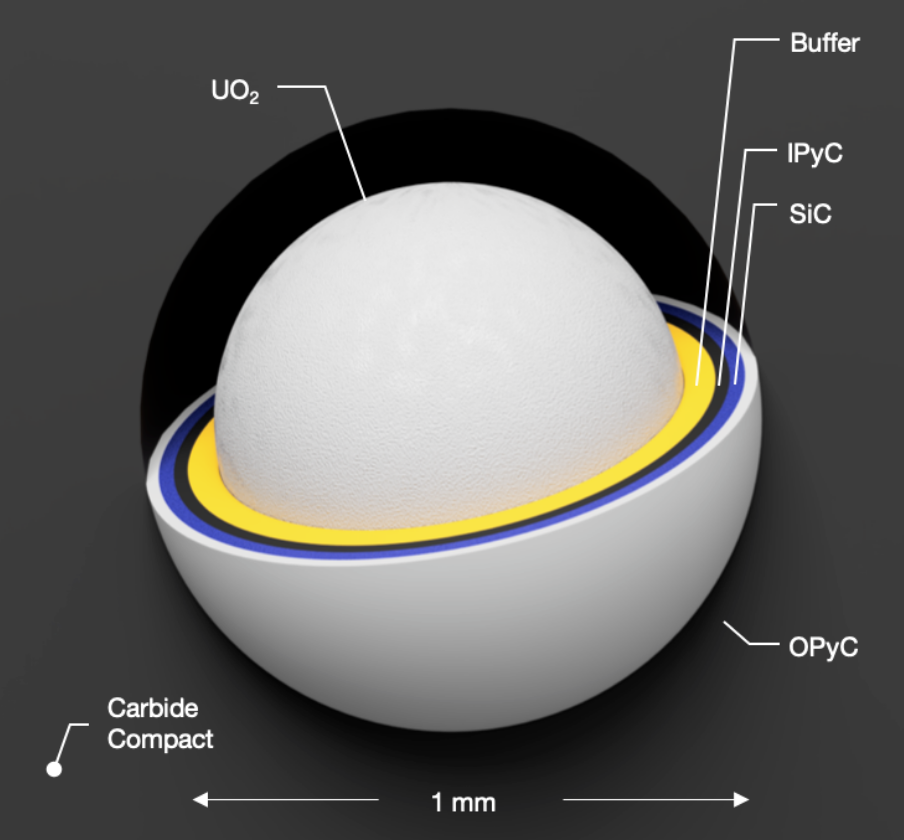
\includegraphics[width=0.5\linewidth]{figures/triso1.png}
	\hfill
	\caption{Typical TRISO particle [Add reference to the website].}
	\label{fig:triso}
\end{figure}

Buffer layer of porous carbon serving as a reservoir for fission gases.
Layers of dense pyrolytic carbon contribute to the mechanical resistance of the particle.
The silicon carbide layer serves as a fission product diffusion barrier.
\cite{france_gas-cooled_2006}